\usetikzlibrary{calc,positioning}
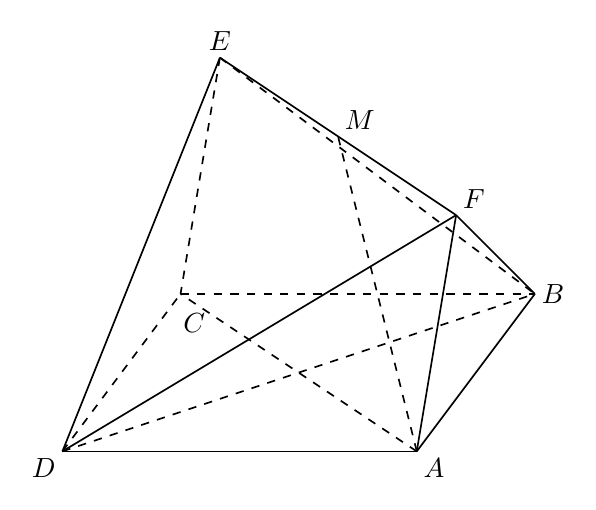
\begin{tikzpicture}[x=1cm,y=1cm,line width=.6pt,font=\normalsize,
 geometry edge/.style={solid,line width=.6pt,draw=black},
 geometry label/.style={font=\normalsize,inner sep=1.5pt,outer sep=1pt,draw=none}]

\coordinate (D) at (0,0);
\coordinate (A) at (4.5,0);
\coordinate (B) at (6,2);
\coordinate (C) at (1.5,2);
\coordinate (E) at (2,5);
\coordinate (F) at (5,3);
\coordinate (M) at (3.5,4);
\draw[geometry edge] (E)--(D);
\draw[geometry edge] (D)--(F);
\draw[geometry edge] (F)--(A);
\draw[geometry edge] (F)--(B);
\draw[geometry edge] (D)--(A);
\draw[geometry edge,dashed] (E)--(C);
\draw[geometry edge] (E)--(F);
\draw[geometry edge,dashed] (D)--(C);
\draw[geometry edge,dashed] (C)--(B);
\draw[geometry edge,dashed] (D)--(B) (A)--(C) (E)--(B);
\draw[geometry edge] (A)--(B);
\draw[geometry edge,dashed] (A)--(M);
\node[geometry label,below left] at (D) {$D$};
\node[geometry label,below right] at (A) {$A$};
\node[geometry label,right] at (B) {$B$};
\node[below right=2pt,xshift=-4.00bp,yshift=-2.00bp] at (C) {$C$};
\node[geometry label,above] at (E) {$E$};
\node[geometry label,above right] at (F) {$F$};
\node[geometry label,above right] at (M) {$M$};
\end{tikzpicture}
